\documentclass{article}
% translate with >> pdflatex -shell-escape <file>

% This file is an extract of the PGFPLOTS manual, copyright by Christian Feuersaenger.
% 
% Feel free to use it as long as you cite the pgfplots manual properly.
%
% See
%   http://pgfplots.sourceforge.net/pgfplots.pdf
% for the complete manual.
%
% Any required input files (for <plot table> or <plot file> or the table package) can be downloaded
% at
% http://www.ctan.org/tex-archive/graphics/pgf/contrib/pgfplots/doc/latex/
% and
% http://www.ctan.org/tex-archive/graphics/pgf/contrib/pgfplots/doc/latex/plotdata/

\usepackage{pgfplots}
\pgfplotsset{compat=newest}

\pagestyle{empty}

\begin{document}
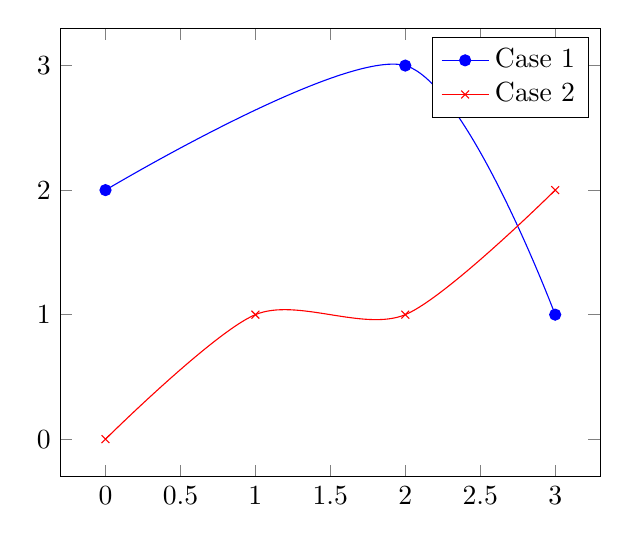
\begin{tikzpicture}
\begin{axis}
\addplot[smooth,mark=*,blue] coordinates {
	(0,2)
	(2,3)
	(3,1)
};
\addlegendentry{Case 1}

\addplot[smooth,color=red,mark=x]
	coordinates {
		(0,0)
		(1,1)
		(2,1)
		(3,2)
	};
\addlegendentry{Case 2}
\end{axis}
\end{tikzpicture}
\end{document}
